%!TEX root = main.tex
\section{evaluation}
\label{sec:eva}

Since evaluation section is where figures and tables appear the most, I put examples of inserting figures and tables here, but they can be used elsewhere.

\subsection{figures}

\begin{figure}[H]
\centering
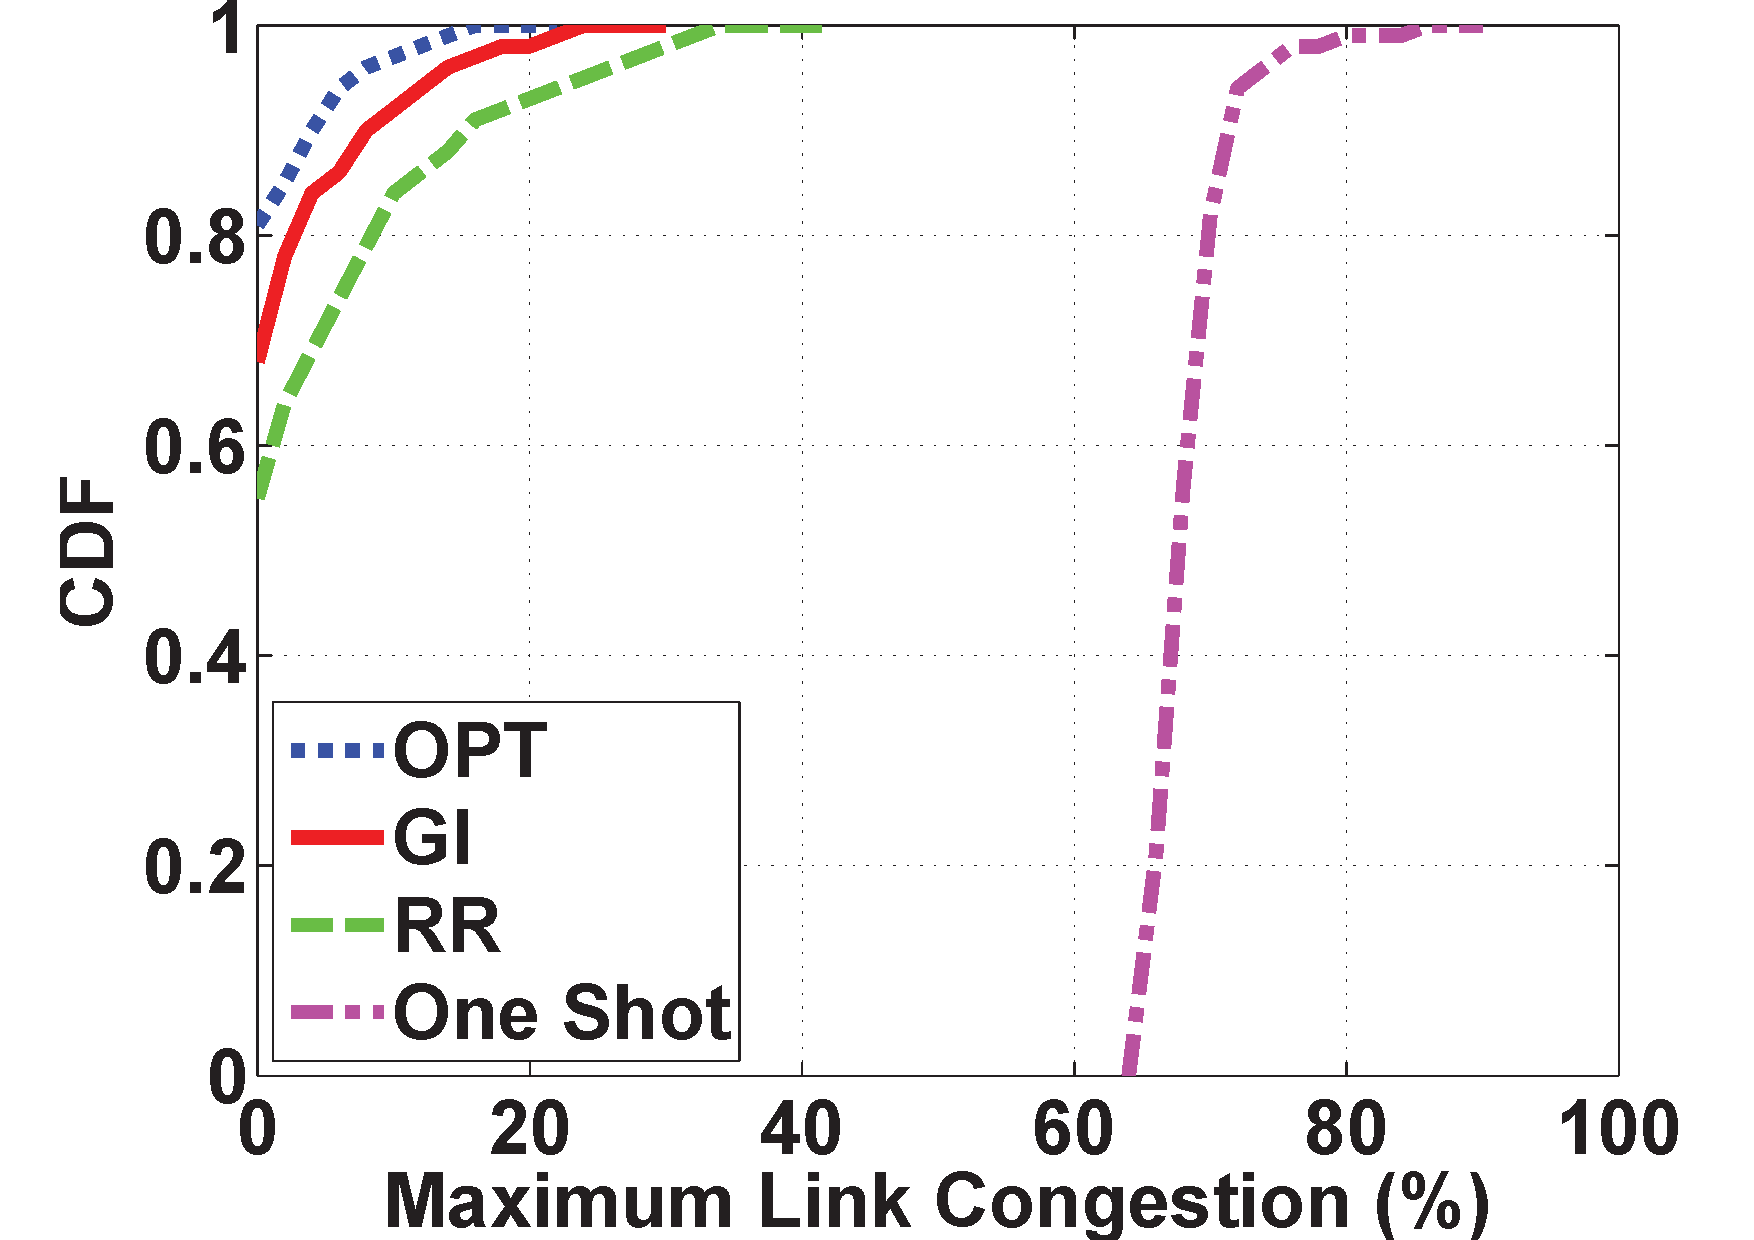
\includegraphics[width=2.0in]{Fig/DCN.pdf}
\caption{insert one figure}
\label{fig:DCN}
\vspace{-3mm}
\end{figure}

\begin{figure}[H]
\subfigure[fig1]{
\begin{minipage}[b]{0.2\textwidth}
\label{fig:TopologyDCN}
\centering
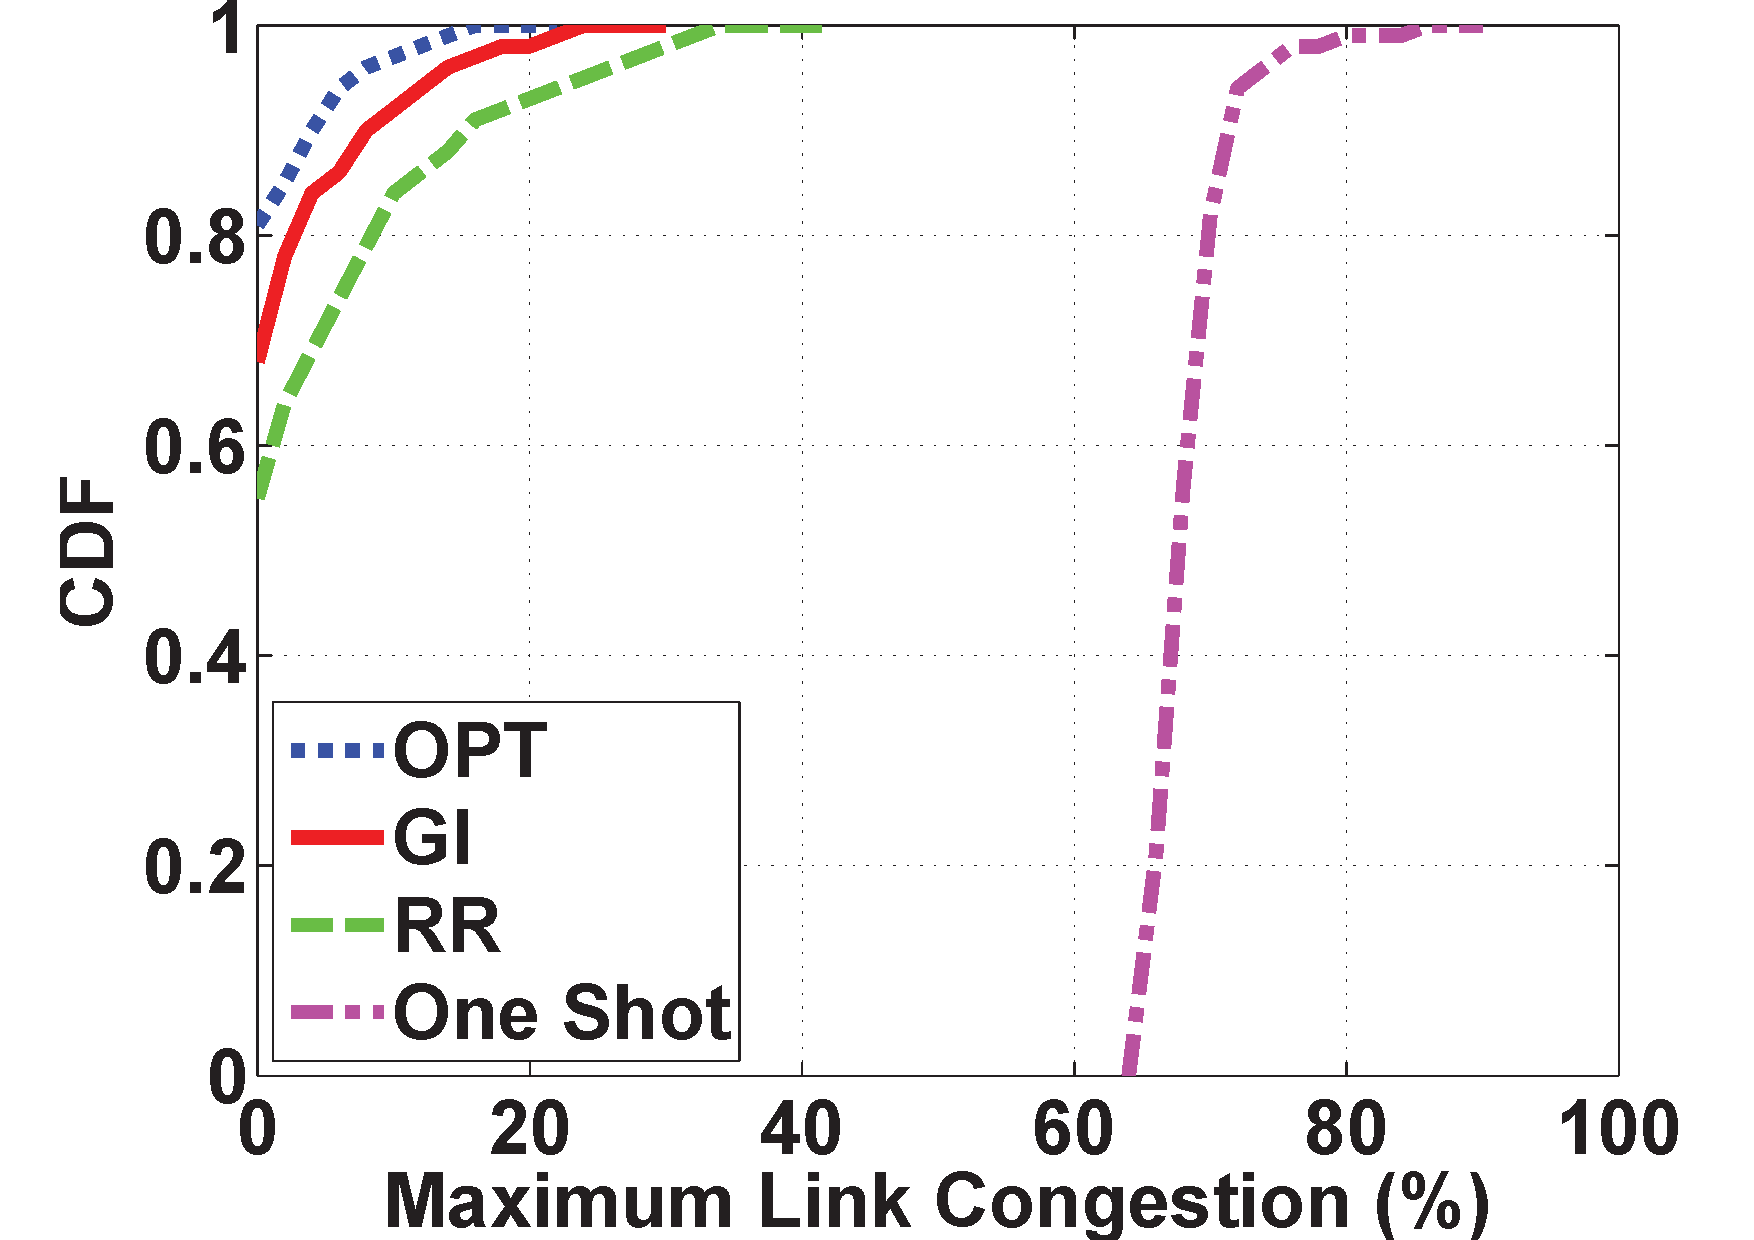
\includegraphics[width=1.5in]{Fig/DCN.pdf}
\end{minipage}}
\subfigure[fig2]{
\begin{minipage}[b]{0.2\textwidth}
\label{fig:TopologyWAN}
\centering
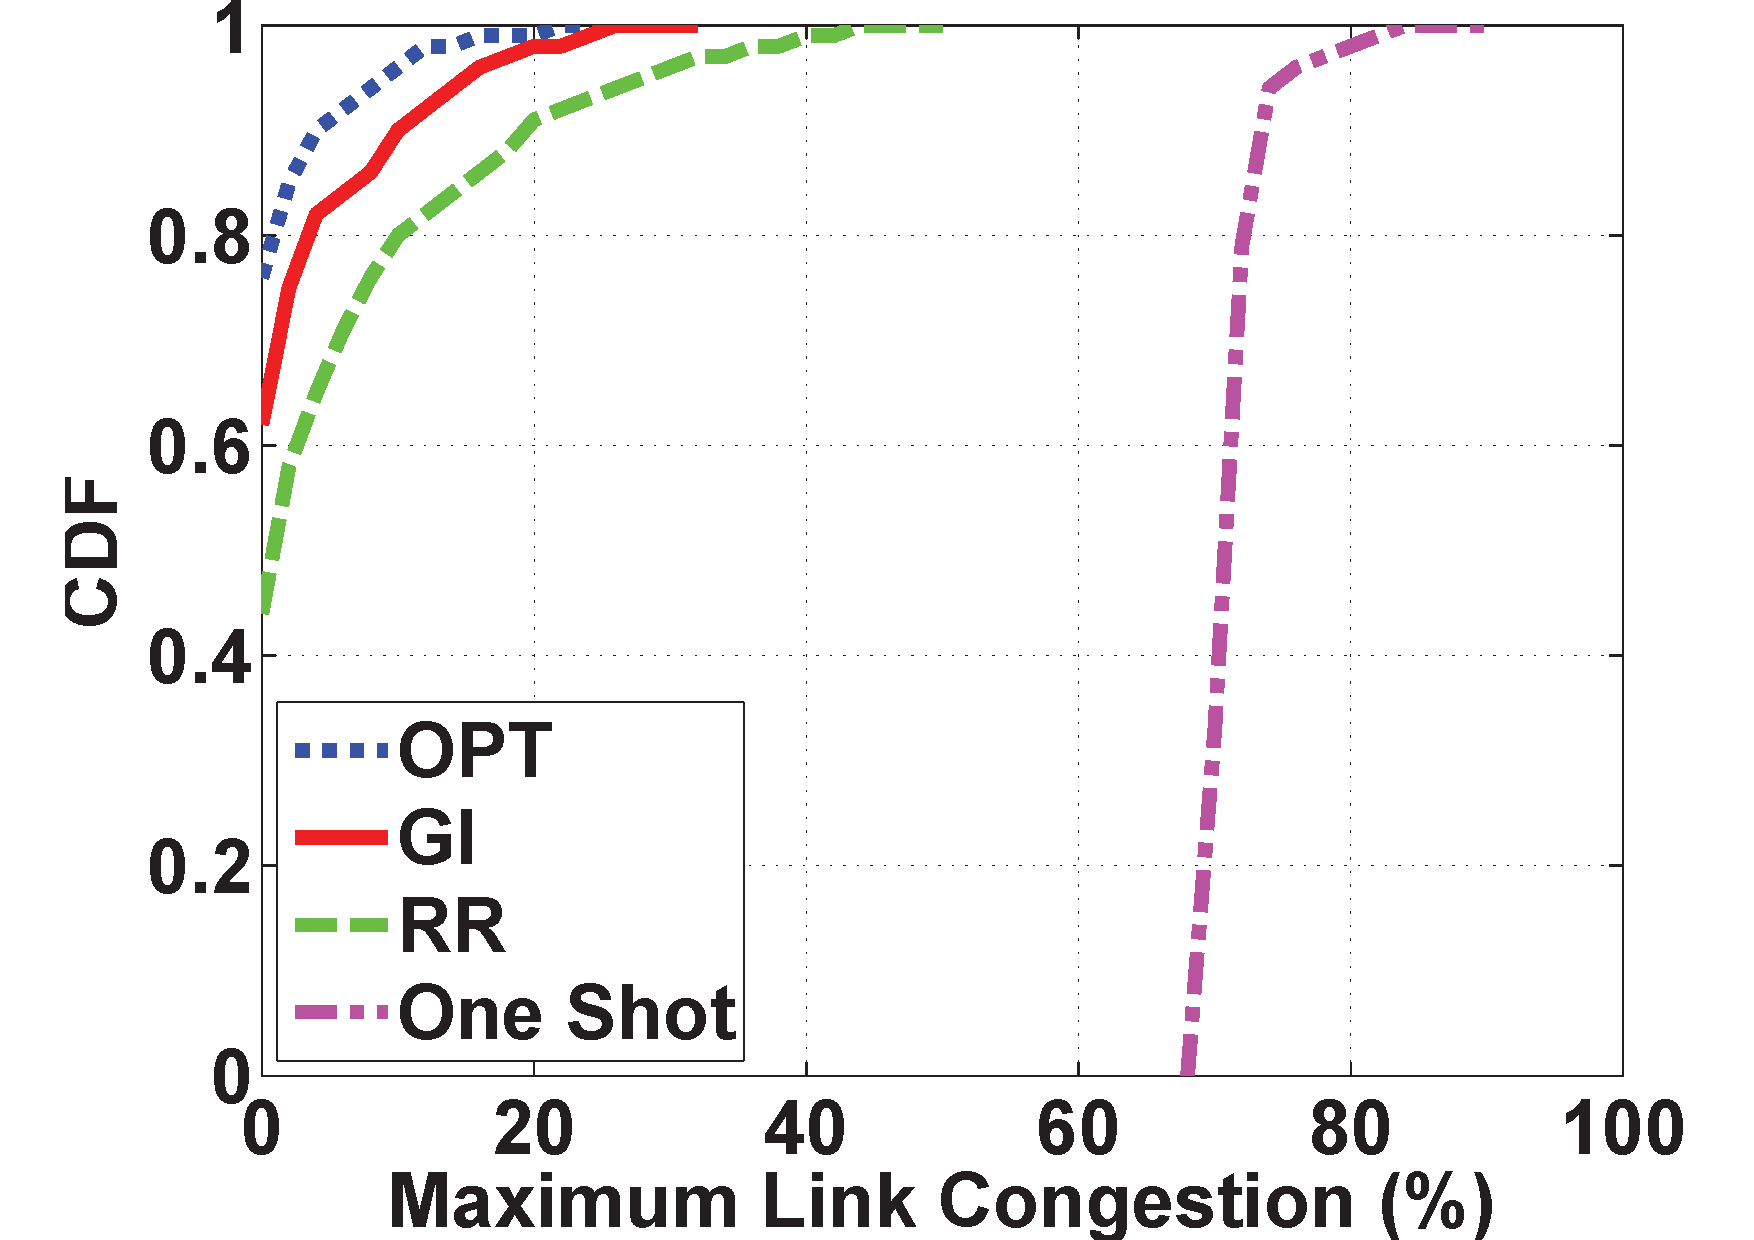
\includegraphics[width=1.5in]{Fig/WAN.pdf}
\end{minipage}}
\caption{put two figures together horizontally} \label{fig:Topology}
\vspace{-1em}
\end{figure}


\begin{figure*}[t]
\begin{minipage}[t]{0.49\textwidth}
\subfigure[DCN scenario]{
\label{fig:DCN}
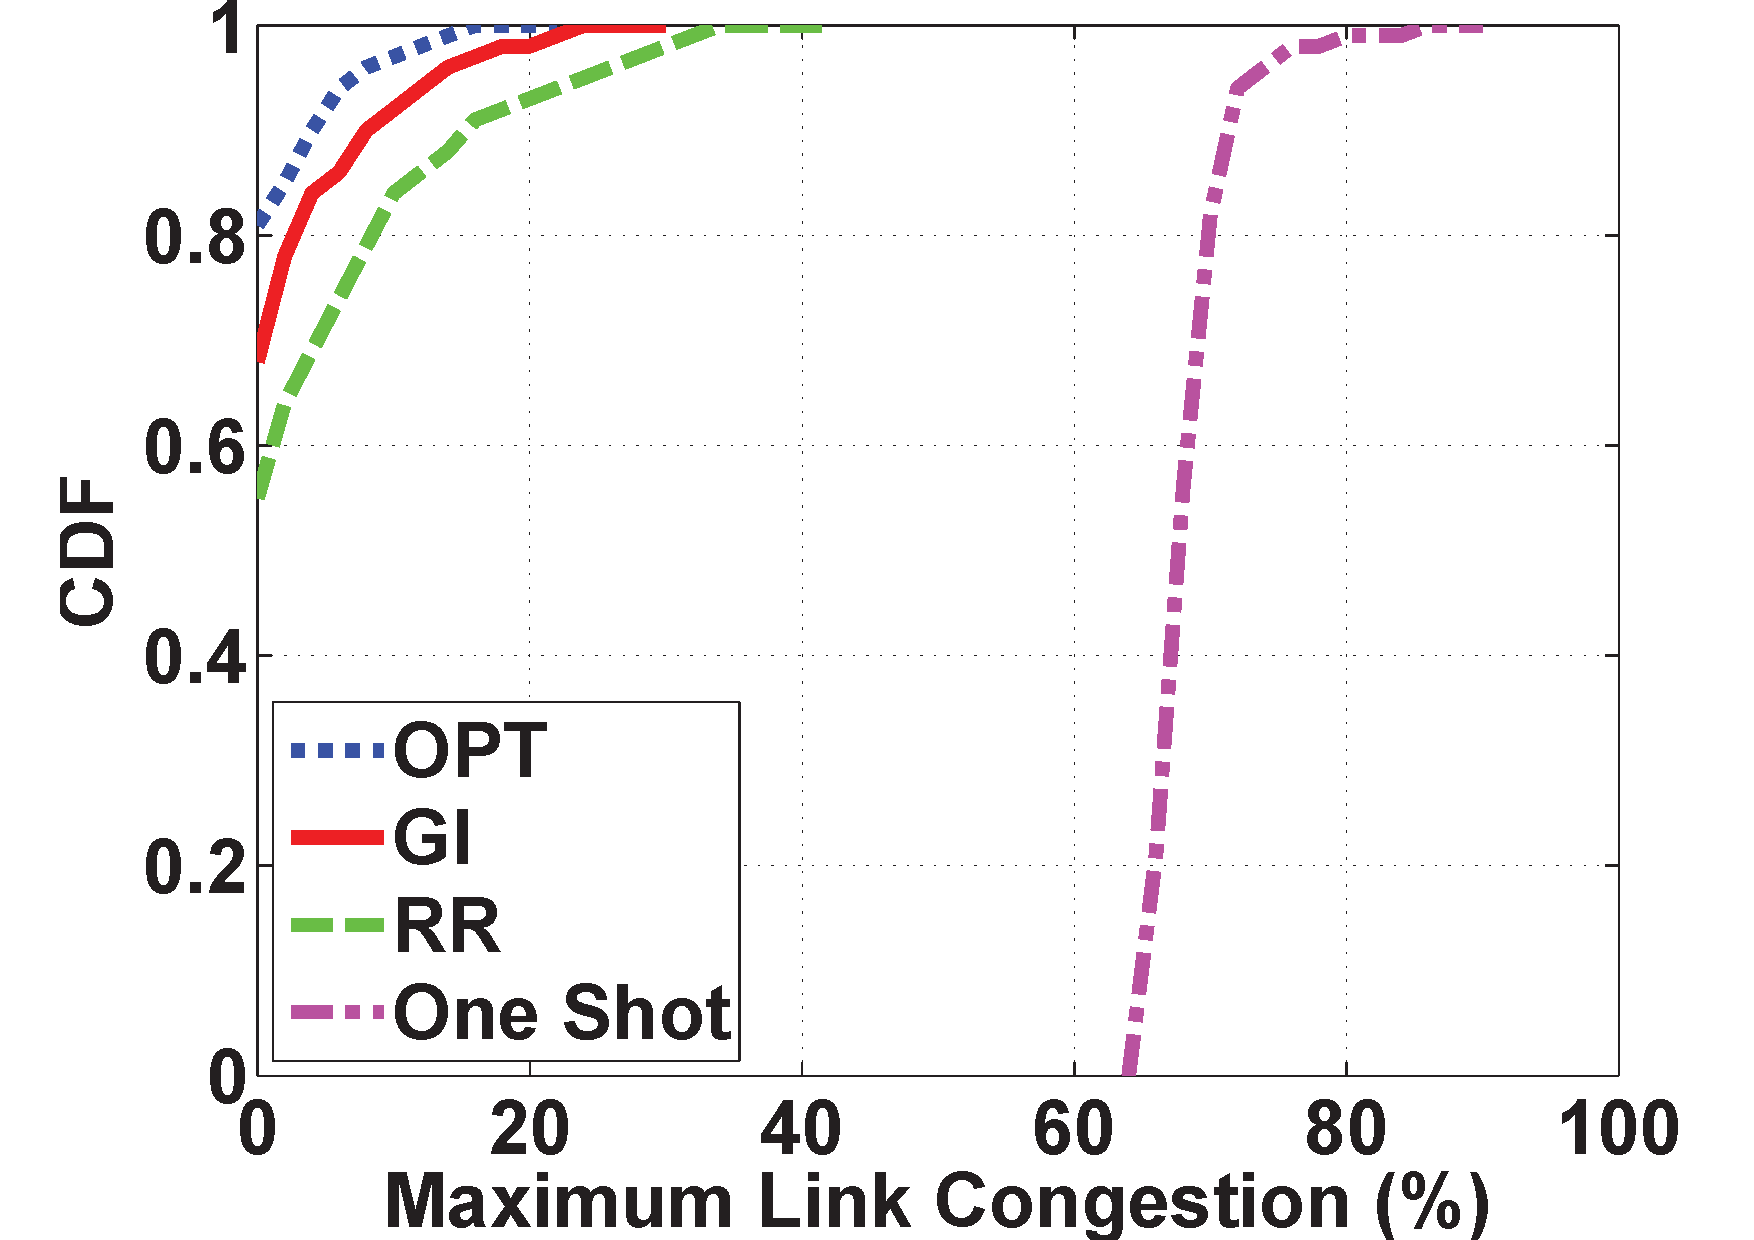
\includegraphics[width=1.6in]{Fig/DCN.pdf}}
\subfigure[WAN scenario]{
\label{fig:WAN}
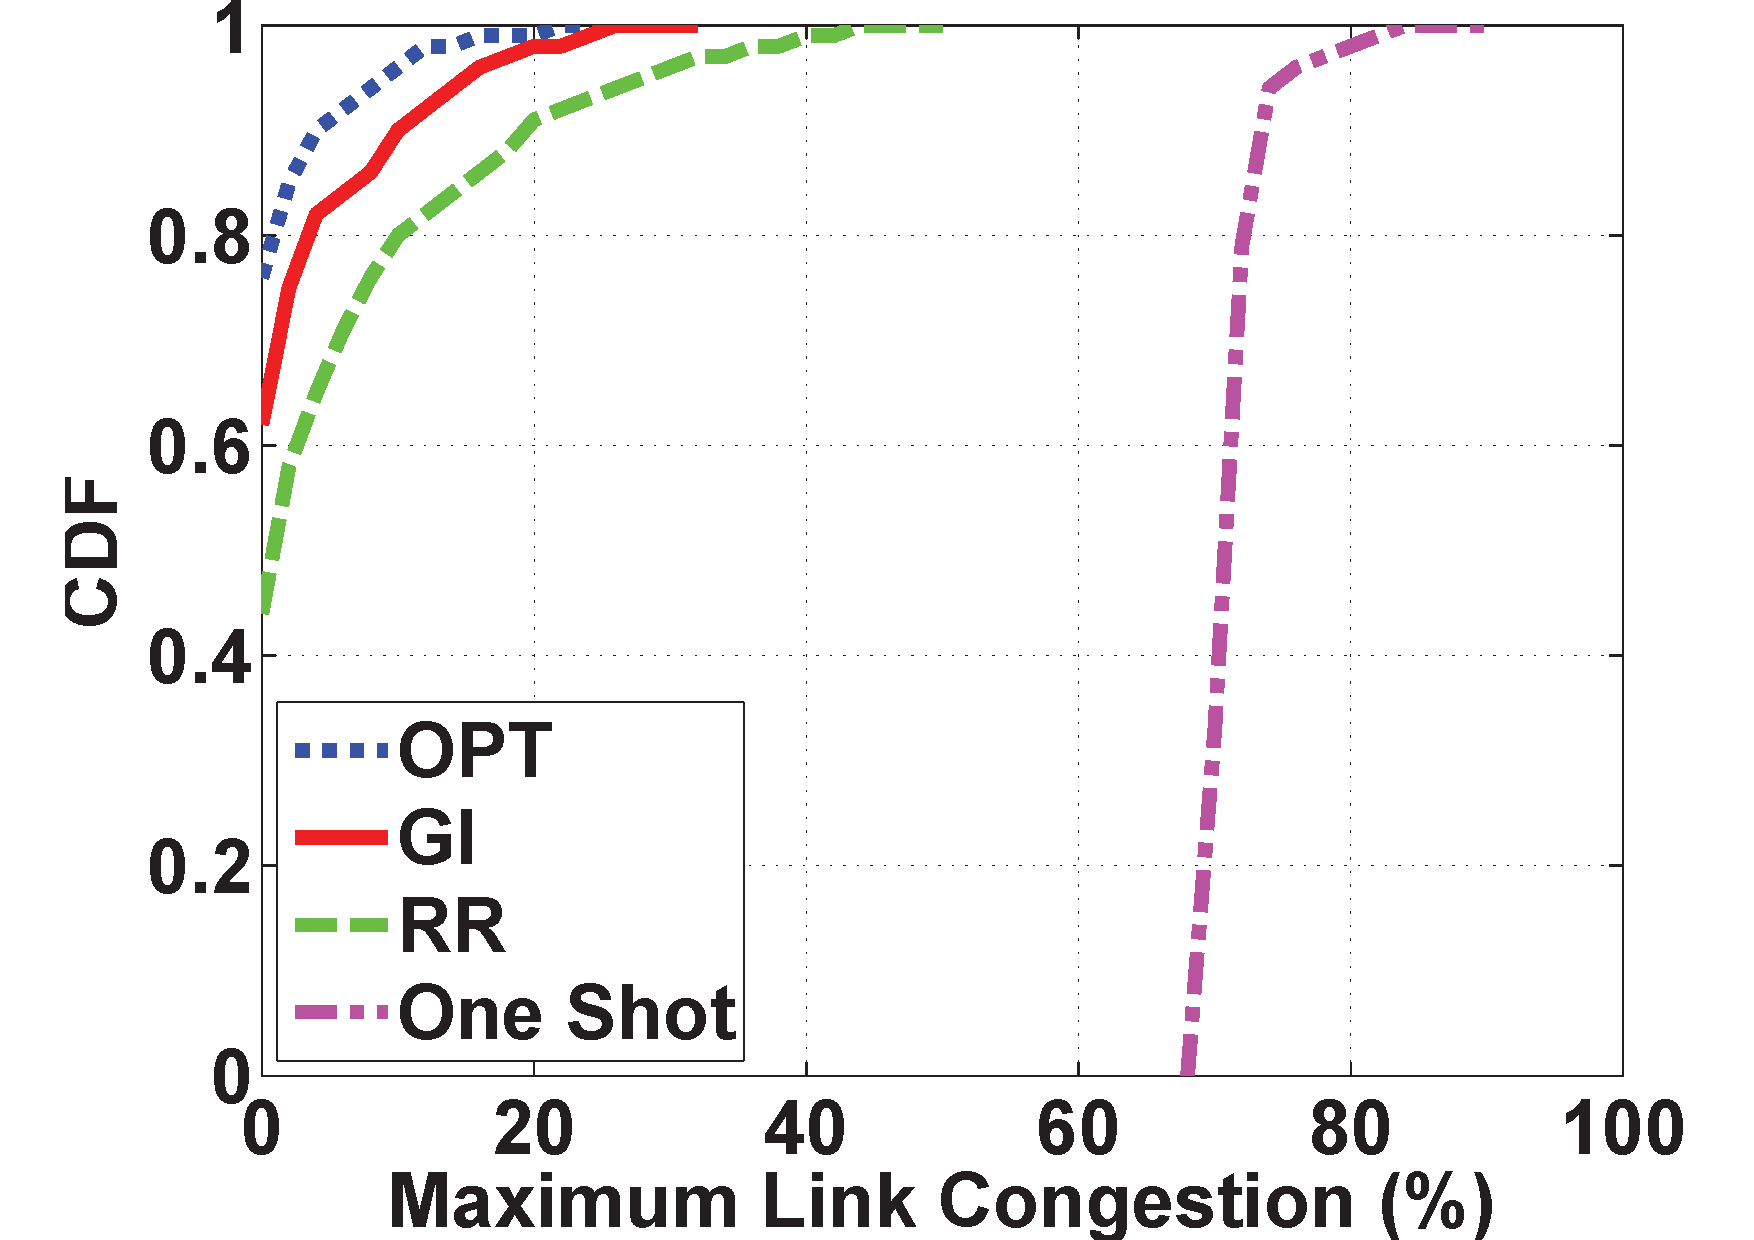
\includegraphics[width=1.6in]{Fig/WAN.pdf}}
\caption{Maximum link congestion comparison.}
\label{fig:LinkCongestion}
\end{minipage}
\begin{minipage}[t]{0.49\textwidth}
\subfigure[DCN scenario]{
\label{fig:RunningTimeDCN}
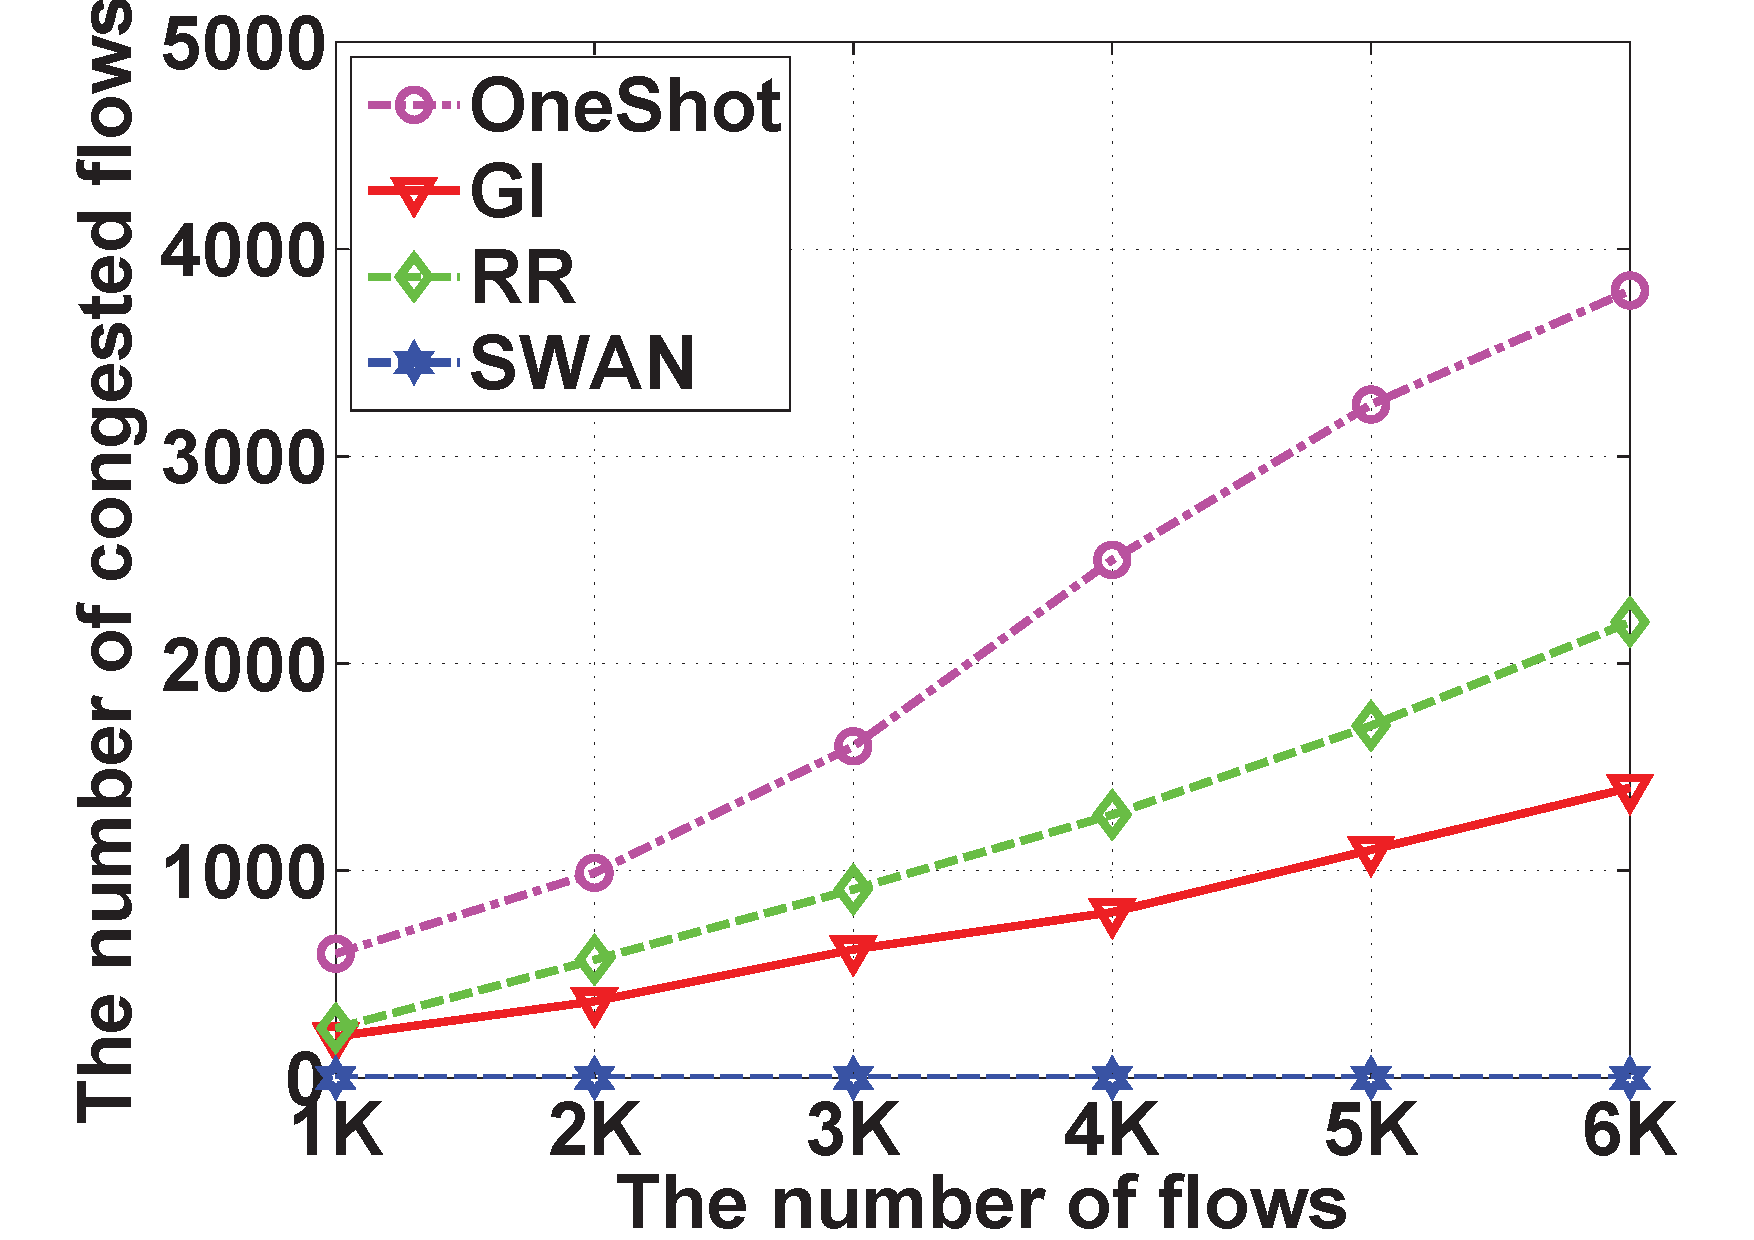
\includegraphics[width=1.6in]{Fig/RTDCN.pdf}}
\subfigure[WAN scenario]{
\label{fig:RunningTimeWAN}
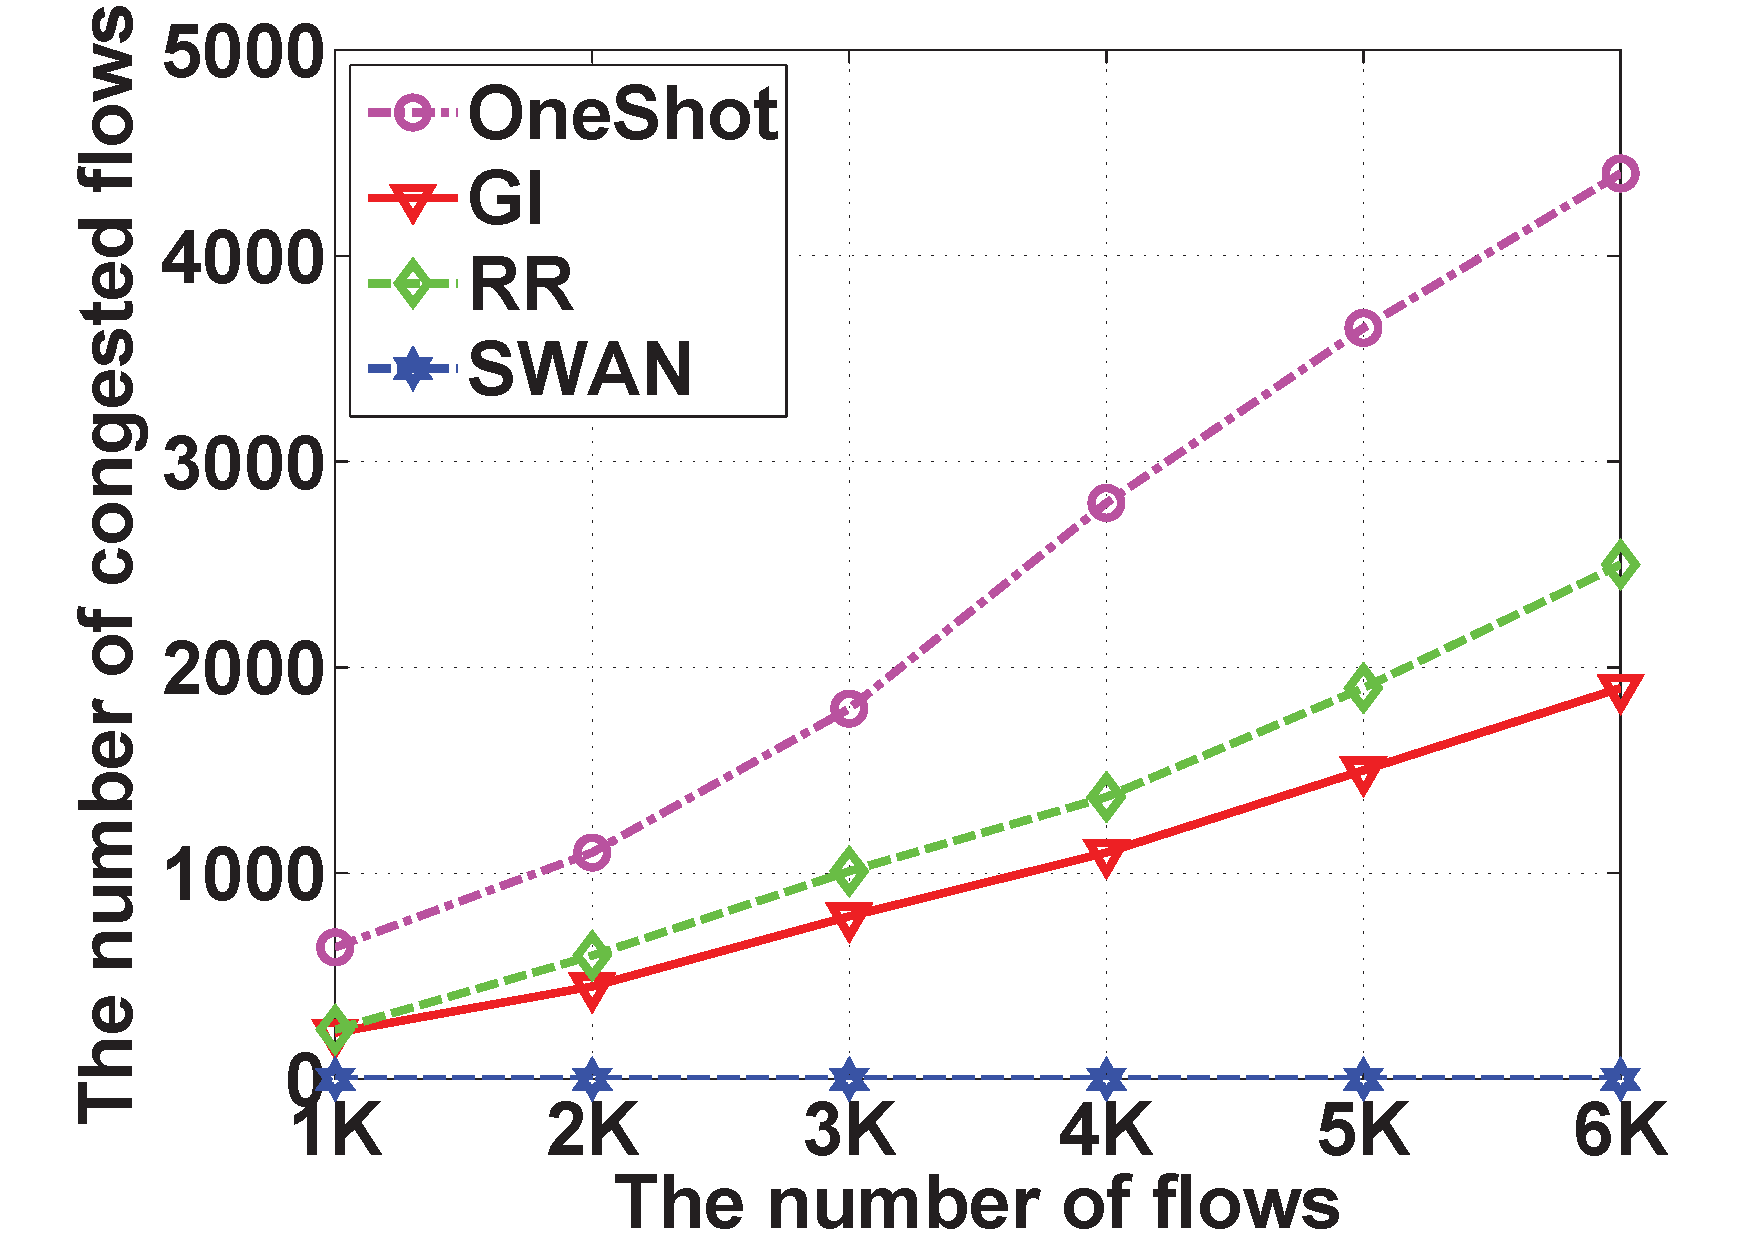
\includegraphics[width=1.6in]{Fig/RTWAN.pdf}}
\caption{The number of congested flows.}
\label{fig:RunningTime}
\end{minipage}
\vspace{-1em}
\end{figure*}

\subsection{tables}

\begin{table}[H]
\caption{Running time for finding congestion-free update plans}\label{Tab:RunningTime}
\centering
\begin{tabular}{|c|c|c|c|c|c|}
\hline
& 1K & 2K & 3K & 4K & 5K  \\
\hline
DCN & 0.73 min & 1.40 min & 2.10 min & 2.96 min &  4.12 min  \\
\hline
WAN & 0.60 min & 1.01 min & 1.57 min & 2.43 min & 3.12 min  \\
\hline
\end{tabular}
\begin{tabular}{l}
\\
write something to explain your table in here
\end{tabular}
\end{table}
